\documentclass[12pt,a4paper]{article}
\usepackage[german]{babel}
\usepackage[T1]{fontenc}
\usepackage[utf8x]{inputenc}
\usepackage{url}
\usepackage{graphicx}
\usepackage{geometry}
\usepackage{amsfonts}
\usepackage{amsmath}
\usepackage{tabularx}
\usepackage{txfonts} %Times New Roman Font
\usepackage{titlesec} %Format der Headings ändern
\usepackage{hyperref}
\usepackage{comment}
\usepackage{listings}
\usepackage{pythonhighlight}

\renewcommand{\thesection}{\arabic{section}.} %Nummerierung der Sections anpassen
\renewcommand{\labelenumi}{\alph{enumi})}  %Nummerierung der Listen anpassen
\titleformat{\section}{\large\bfseries}{\thesection}{0.5em}{} %Format der Section Überschrift ändern
\setlength{\parindent}{0pt} %Keine Einrückung bei neuen Paragraphen
\geometry{left=2.0cm,textwidth=17cm,top=2.5cm,textheight=23cm}

% Anpassen %
%%%%%%%%%%%%%%%%%%%%%%%%%%%%%%%%%%%%%
\newcommand{\student}{Daniel Pantjuskin-Moos\\ 108013248222 } % Namen eintragen
\newcommand{\partner}{Vincent König\\ 108011232630} % Matrikelnummer eintragen
\newcommand{\group}{D} % Gruppennummer eintragen
%%%%%%%%%%%%%%%%%%%%%%%%%%%%%%%%%%%%%

\newcommand{\hwheadtwo}{$ $
  \vspace{-2cm}
  
\noindent \student \qquad \qquad  Wireless Physical Layer Security Praktikum \hfill SS 2020 \\
\noindent \partner \\
%\noindent \thirdone \\  % einkommentieren, falls ihr eine 3er Gruppe seid
\noindent Gruppe:~\group\\
$ $

  
\begin{center}    
{\Large \bf Abgabe PHYSEC 3}
\end{center}
}

\begin{document}
\hwheadtwo

\section{Messungen}

\section{Implementierung Pearson Correlation}


Die Aufgabenstellung ist, die in Abbildung~\ref{fig:Label1}
abgebildete Formel in einem vorgegeben Python-Code als Funktion 
\textit{correlation(X, Y)} zu implementieren, sodass es von einem 
mitgegeben Framework fehlerlos getestet werden kann. 
Die vollständige \textit{exercise3.py} kann  
\href{https://mega.nz/file/7gwx0BwR#dwkLdHX7AglZKYwp9poGQ-tEL20GtaqFy8LoT4TtV_g}
{hier} 
heruntergeladen werden.

\begin{figure}[hbt!]
	\centering
		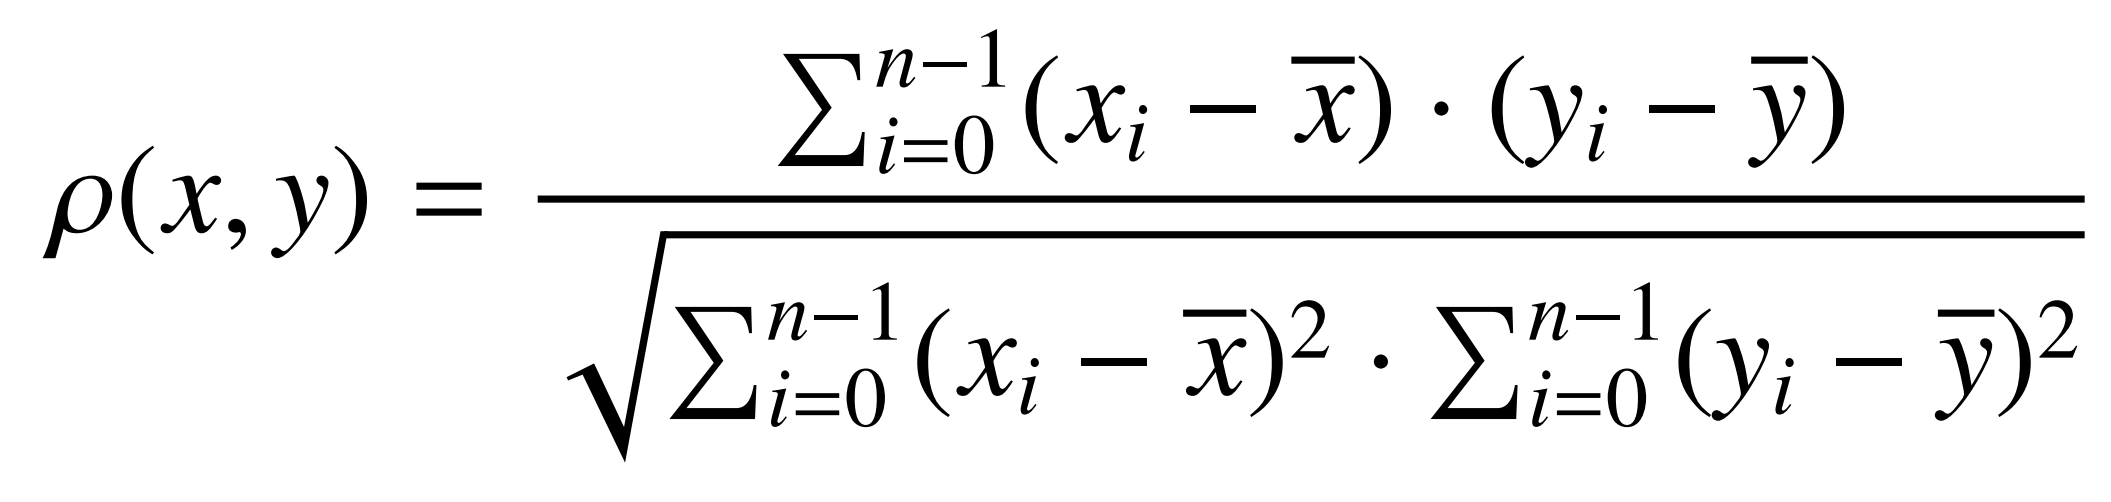
\includegraphics[width=1\textwidth ]
		{Bilder/a2-pearson-formel.png}
		\caption{Auszug aus dem Assignment}
		\label{fig:Label1}
\end{figure}

\begin{python}

import utils
import numpy

"""
Excersise 3:
Implement the Pearson correlation coefficient.
Do NOT use any given function for standard-deviation 
or mean-value but implement them by yourself.

X, Y are given as lists.

Blockwise application is done outside so please use the 
whole vectors at once.
"""


def correlation(X, Y):
    mean_x = numpy.mean(X) # Mittel Vektor X
    mean_y = numpy.mean(Y) # Mittel Vektor Y

    numerator = 0 # zaehler
    denominator_x = 0 # der X beinhaltene Faktor im Nenner
    denominator_y = 0 # der Y beinhaltene Faktor im Nenner

    # Falls Vektoren unterschiedlich lang sind
    if len(X) != len(Y):
        raise Exception("Length not equal!\n")

    for i in range(len(X)):
        numerator += (X[i] - mean_x)*(Y[i] - mean_y)
        denominator_x += (X[i]-mean_x)*(X[i]-mean_x)
        denominator_y += (Y[i]-mean_y)*(Y[i]-mean_y)

    denominator = numpy.sqrt(denominator_x * denominator_y)

    # Falls Nenner=0, dann wird der jeweilige Eintrag ignoriert
    # und wird somit auch nicht in die Skizzen eingetragen
    if denominator == 0:
        return float('nan')

    pearson = numerator/denominator

    return pearson
    # return utils.not_yet_implemented("Correlation")

\end{python}

\section{Auswertung}

\section{Quantisierer Jana Multibit}

\section{Quantisierer Mathur Suhas}

\section{Bonus: Reading Assignment}



\begin{comment}
% Beispiel für einen Hyperlink 	
\href{https://www.rub.de}{hier klicken}

% Beispiel für Bilder mit Caption und Referenz

\begin{figure}[hbt!]
	\centering
		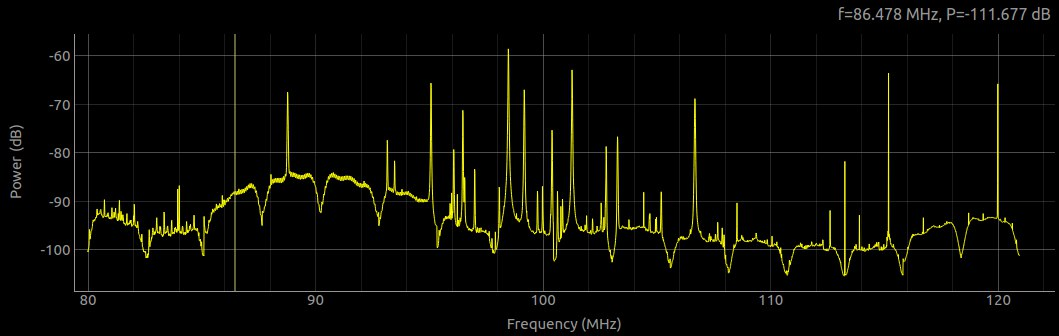
\includegraphics[width=1\textwidth ]
		{Bilder/a3_rtl_sdr.jpg}
		\caption{Hier Caption einfügen}
		\label{fig:Labelx}
\end{figure}

% Als Beispiel wie man referenziert
~\ref{fig:Labelx}

% Beispiel für das Einfügen von Python Code
\begin{python}
print("Hello World")
\end{python}

% Beispiel für das Erzwingen von Abstand 
\hspace{0.5mm}

\end{comment}

\end{document}